\documentclass[a4paper]{article}

\usepackage{graphicx}
\usepackage{float}
\usepackage{hyperref}
\usepackage{xcolor}
\usepackage[spanish]{babel}
\usepackage{listings}
\usepackage{enumitem}
\usepackage[utf8]{inputenc}

\lstset{language=c, frame=tlrb, basicstyle=\scriptsize, breaklines=true, numberbychapter=false,numbers=left}
\setlist[enumerate]{noitemsep}
\setlist[itemize]{noitemsep}

\begin{document}

\title{Infraestructura de Análisis de Rendimiento\\
\bigskip
{\large Propuesta de tesis para\\} Magister en Cómputo de Altas Prestaciones\\
\bigskip
Universidad Nacional de La Plata\\
Facultad de Informática\\
\bigskip
}

\author{Tesista: Andrés More - {\tt amore@hal.famaf.unc.edu.ar}\\
Director: Dr. Fernando G. Tinetti - {\tt fernando@lidi.info.unlp.edu.ar}}

\date{Agosto de 2013}

\maketitle

\newpage

\section{Objetivo}

La propuesta principal consiste en el desarrollo de una infraestructura de soporte para el análisis de rendimiento en aplicaciones de cómputo de altas prestaciones.

\bigskip

La infraestructura a desarrollar implementará un procedimiento sistemático de análisis de rendimiento ejecutando pruebas de referencia, herramientas de perfil de rendimiento y análisis de resultados.  La infraestructura generará como resultado final un informe detallado para soportar la tarea de optimización con información cuantitativa. El reporte final incluirá datos estadísticos de la aplicación y el sistema donde se ejecuta, además de gráficos de desviación de resultados, escalamiento de problema y capacidad de cómputo e identificación de cuellos de botella.

\section{Motivación/Estado del Arte del Tema}

En el área de HPC los programadores son los mismos especialistas del dominio del problema a resolver. Las rutinas
más demandantes de cálculo son en su mayoría científicas y su alta complejidad hace posible su correcta implementación sólo por los mismos investigadores. Estas cuestiones resultan en un tiempo reducido de optimización de rendimiento
e impactan directamente en la productividad de los grupos de investigación y desarrollo. Frecuentemente el proceso de optimización termina siendo hecho de modo {\it ad-hoc}, sin la utilización de información cuantitativa para dirigir los
esfuerzos de mejora.

\bigskip

Algunas referencias a la problemática se incluyen a continuación como soporte de la propuesta:

\begin{enumerate}

\item Cómo correctamente mostrar resultados de rendimiento por {\it Fleming, Philip J. and Wallace, John J.} en {\it How Not to Lie with Statistics: the Correct Way to Summarize Benchmark Results}, {ACM}, {29/3}, {1986}.

\item Cómo acceder a memoria eficientemente por {\it Drepper, Ulrich} en {\it What Every Programmer Should Know About Memory}, Reporte Técnico, 2007.

\item Una discusión de la dificultad de la programación en paralelo por {\it McKenney, Paul E.} en {\it Is Parallel Programming Hard, And, If So, What Can You Do About It?}, Reporte Técnico, 2007.

\item Una revisión de como medir rendimiento durante el desarrollo de una aplicación por {\it Woodside, Murray and Franks, Greg and Petriu, Dorina C.} en {\it The Future of Software Performance Engineering}, IEEE Computer Society, 2007.

\item Ejemplos de optimización compleja por {\it Jeff A. Bilmes et al.} en {\it BLAS3 Compatible Fast Matrix Matrix Multiply} y también por {\it R. Clint Whaley et al.} en {\it Automatically Tuned Linear Algebra Software}, ICSI, 1998.

\item Cómo utilizar información de contadores de hardware durante la ejecución de un programa por {\it Thomas Ball} en {\it Eficiently counting program events with support for on-line queries}, ACM Programming Languages and Systems, 1994.

\item Cómo optimizar software teniendo en cuenta arquitectura de bajo nivel por {\it Intel} en {\it Intel® 64 and IA-32 Architectures Optimization Reference Manual}, Intel Press, 2013.

\end{enumerate}

En principio el desarrollo se limita al soporte de ambientes {\it GNU/Linux}, con aplicaciones utilizando paralelismo implementado utilizando tecnología {\it OpenMP}.

\section{Temas de Investigación}

Esta sección contiene una lista inicial de los temas a trabajar:

\begin{description}
\item[Configuración y ejecución de pruebas de referencia:]

Las pruebas de rendimiento proveen una línea base de comparación sobre las capacidades de los diferentes componentes de un sistema de cómputo, ya sea aislados o trabajando en conjunto. Las principales candidatas son {\it HPCC} y {\it HPL}.

\item[Aplicación general de herramientas de perfil de ejecución:]

Un perfil de ejecución de una aplicación permite conocer su comportamiento interno, identificando que partes necesitan ser optimizadas. El perfil puede ser construido utilizando instrumentación del código e incluso utilizando soporte de contadores de {\it hardware}.

\item[Generación de gráficos de rendimiento:]

Los gráficos facilitan el análisis y modelado del comportamiento de una aplicación. Por ejemplo: un histograma de la distribución de resultados permite entender la desviación de los mismos, un gráfico histórico comparando diferentes versiones de una aplicación permite comprobar mejoras, un gráfico de tiempos de ejecución permite entender escalamiento de una aplicación.

\item[Análisis diferencial de rendimiento:]

La comparación histórica de resultados permite corroborar los resultados de las diferentes optimizaciones.

\item[Optimización guiada por perfil de ejecución:]

La mayoría de los compiladores actuales permiten utilizar información de una ejecución previa para optimizar el acceso a instrucciones en cache de instrucciones y datos en sus diferentes niveles.

\item[Monitorización utilizando Contadores de Eventos en Hardware:]

Los contadores a nivel de {\it hardware} ofrecen mayor precisión, evitan errores de muestreos y producen menor sobrecarga que instrumentar {\it software}.

\item[Generación de reportes:]

Como soporte para el análisis de rendimiento, se incluye como resultado final un reporte integral con información de referencia, datos de perfil de ejecución y gráficos de rendimiento. Identificando problemas y áreas de mejora potenciales.

\end{description}

\section{Desarrollos/Trabajo Experimental a Realizar}

La infraestructura a desarrollar consiste de distintos componentes, como se demuestra en la Figura \ref{fig:framework} a continuación.

\begin{figure}[H]
\centering
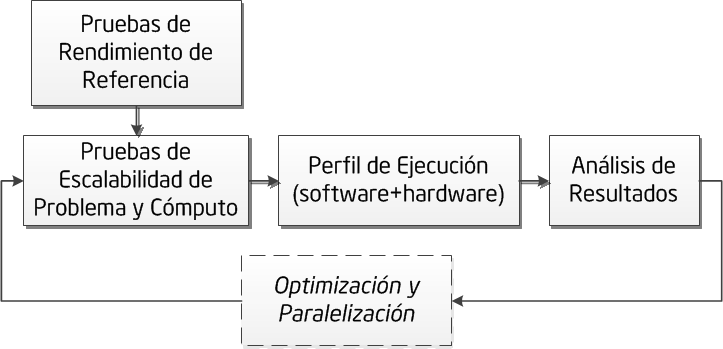
\includegraphics[width=8cm]{framework.png}
\caption{Infraestructura a Desarrollar}
\label{fig:framework}
\end{figure}
  \begin{description}
  \item[Pruebas de Rendimiento de Referencia:] automáticamente configura y ejecuta pruebas sobre el sistema, publicando números de rendimiento relevantes.
 \item[Pruebas de Escalabilidad:] se ejecuta la aplicación variando tamaño de problema y también capacidad de cómputo para obtener información de comportamiento y límites de escalabilidad.
  \item[Perfil de Ejecución:] automáticamente configura y ejecuta herramientas para medir rendimiento e identificar cuellos de botella en una aplicación utilizando soporte de {\it software} y {\it hardware}.
  \item[Análisis de Resultados:] utilizando la información anterior, calcula límites de potenciales mejoras y lista los cuellos de botella principales asociados al código de la aplicación.
  \item[Generación de reporte:] a partir de la información anterior, compila un reporte incluyendo gráficos y referencias al código específico a optimizar.
  \end{description}

La tarea de optimización y paralelización entonces es realizada manualmente, utilizando información estadística y cuantitativa sobre el comportamiento de la aplicación, extraída automáticamente por la infraestructura a desarrollar.

\section{Esquema de Plan de Trabajo}

El siguiente cronograma muestra el plan de actividades tentativo incluyendo actividades y tiempos.

\begin{table}[H]
  \caption{Detalle de Actividades}
  \centering
    \begin{tabular}{|l|l|}\hline
      {\bf Actividad} & {\bf Duración} \\ \hline
	Estado del Arte & Octubre \\ \hline
      Diseño de Alto Nivel & Noviembre \\ \hline
      Prototipo & Diciembre-Enero-Febrero \\ \hline
      Pruebas de Rendimiento & Marzo \\ \hline
      Cálculo de Leyes & Abril \\ \hline
      Perfil de Rendimiento & Mayo-Junio-Julio \\ \hline
      Eventos y Vectorización & Agosto \\ \hline
      Documentación Tesis & Septiembre-Octubre \\ \hline
    \end{tabular}
  \label{schedule}
\end{table}

\section{Posibilidades de Realización}

El alumno tiene a su disposición acceso al equipamiento necesario como parte de su ámbito laboral.
El alumno trabaja como Ingeniero en Software en {\it Argentina Software Design Center} (ASDC - Intel Córdoba); también
como docente e investigador en el Instituto Universitario Aeronáutico dictando tanto cursos de grado (Cómputo de Altas Prestaciones) como postgrado (Implementación de Sistemas Operativos).

\section{Bibliografía Básica Relacionada}

Un conjunto inicial a modo de referencia es incluido en la bibliografía listada a continuación.

\begin{thebibliography}{9}
  
\bibitem{critical-overview}
 J. Browne,
 \emph{A critical overview of computer performance evaluation},
 1976.

\bibitem{patterns}
 G. Mattson, B.A. Sanders and B.L. Massingill, 
 \emph{Patterns for Parallel Programming, Addison-Wesley},
 2004.

\bibitem{automatic-performance-analysis}
 T. Margalef, J. Jorba, O. Morajko, A. Morajko, E. Luque,
 \emph{Different approaches to automatic performance analysis of distributed applications},
 2004.

\bibitem{intro-software-performance}
 C. Smith,
 \emph{Introduction to software performance engineering: origins and outstanding problems},
 2007.

\bibitem{future-software-performance}
 M. Woodside, G. Franks, D. Petriu,
 \emph{The Future of Software Performance Engineering},
 2007.

\bibitem{capturing-performance-knowledge}
 K. Huck, O. Hernandez, V. Bui, S. Chandrasekaran, B. Chapman, A. Malony, L McInnes, B. Norris,
 \emph{Capturing performance knowledge for automated analysis},
 2008.

\bibitem{spec}
  Andres More,
 \emph{Herramientas de Soporte para Análisis de Rendimiento},
 Trabajo Final Especializacion HPC/GRID - UNLP 2013.

\bibitem{counters}
  Fernando G. Tinetti, Mariano Mendez, and Armando De Giusti,
  \emph{An Automated Approach to Hardware Performance Monitoring Counters},
  2013. 

\bibitem{openmp}
  OpenMP Architecture Review Board,
  \emph{OpenMP Application Program Interface Version 3.0},
  Mayo 2008.

\end{thebibliography}

\end{document}
